
\subsection{Ontología del dominio} \label{sec:ontologia}

El conocimiento adquirido para este problema se representa mediante una
ontología. En esta aparecen todos los conceptos detallados en la
\autoref{sec:conceptualizacion} y las relaciones entre ellos, puesto que debe
permitir al sistema basado en el conocimiento razonar sobre ellos de forma
adecuada. Para formalizarlos, deberemos pensar en una forma para representarlos
y que nuestro sistema basado en el conocimiento lo entienda. A continuación, 
pasamos a detallar las partes principales de la ontología desarrollada.

La ontología empieza con el Alumno que se podrá distinguir según su DNI.
Desde él podremos acceder a todo su expediente de las asignaturas a las
que se ha presentado y a sus preferencias sobre cómo le gustaría que fuese su
próxima elección de matrícula. Esto nos sirve para que desde la clase Alumno
podamos gestionar sus preferencias y restricciones o inferirlas si es
necesario y así poder escoger las mejores asignaturas para una buena recomendación.

El expediente único del alumno tendrá todas las convocatorias de exámenes
del alumno. Para distinguir una convocatoria usaremos la asignatura y el
cuatrimestre en el que se ha presentado. Esto nos permitirá que un alumno
se pueda presentar a la misma asignatura en más de una ocasión si éste la
suspendiera. Como atributos tendremos la calificación y su horario.

Las asignaturas son los conceptos que permanecerán estáticos durante toda
la ejecución del sistema. Su conocimiento no podrá ser modificado por el
alumno porque es independiente de él y es algo nos proporciona la Facultad.
Cada asignatura consistirá en un nombre (tomaremos sus siglas para abreviar),
el curso en el que aparece en el plan de estudios, su número de créditos
ECTS (así como la distribución en horas de esta carga por los conceptos de
teoría, problemas y laboratorio), el horario de impartición y si la asignatura
consiste en un proyecto. También incluirá las estadísticas más recientes
referentes al número de alumnos matriculados y el porcentaje de aprobados; y la
relación de la asignatura con las competencias que desarrolla y con los temas
en los que se ubica su contenido. Además, modelamos para cada asignatura las
dependencias con otras asignaturas en forma de prerrequisitos, correquisitos,
precorrequisitos y orrequisitos.
%%% TODO: quizá describir brevemente cada tipo de requisito %%%
A partir de la clase Asignatura se derivan tres clases que representan los
diferentes tipos de asignaturas del plan de estudios: Especializada para
las asignaturas de especialidad (contiene un atributo adicional que indica
la especialidad a la que pertenece), Obligatoria para las asignaturas troncales
y Optativa para las asignaturas de carácter opcional.
%%% TODO: citar acta académica %%%

Para poder tener acceso a las preferencias y restricciones hemos decidido
agruparlos en un solo concepto porque la información que debemos obtener es
la misma para ambas, pero con un matiz distinto. Para distinguir entre cada
uno tendremos un atributo booleano esPreferencia que  nos indica si se ha
de cumplir siempre (restricción) o si no es algo primordial el que se cumpla
(preferencia). Heredado de él tendremos un subconcepto para cada
preferencia/restricción que se quiera introducir en el sistema. Para poder
diferenciarlos, usaremos el atributo booleano y su subconcepto. De este modo
podremos tener una restricción y una preferencia de un mismo subconcepto.

En la \autoref{fig:ontologia-completa} se muestra el esquema de la jerarquía 
de la ontología anteriormente descrita.

\afterpage{% Página horizontal (a parte).
\begin{landscape}

    \begin{figure}[ht]
        \centering
        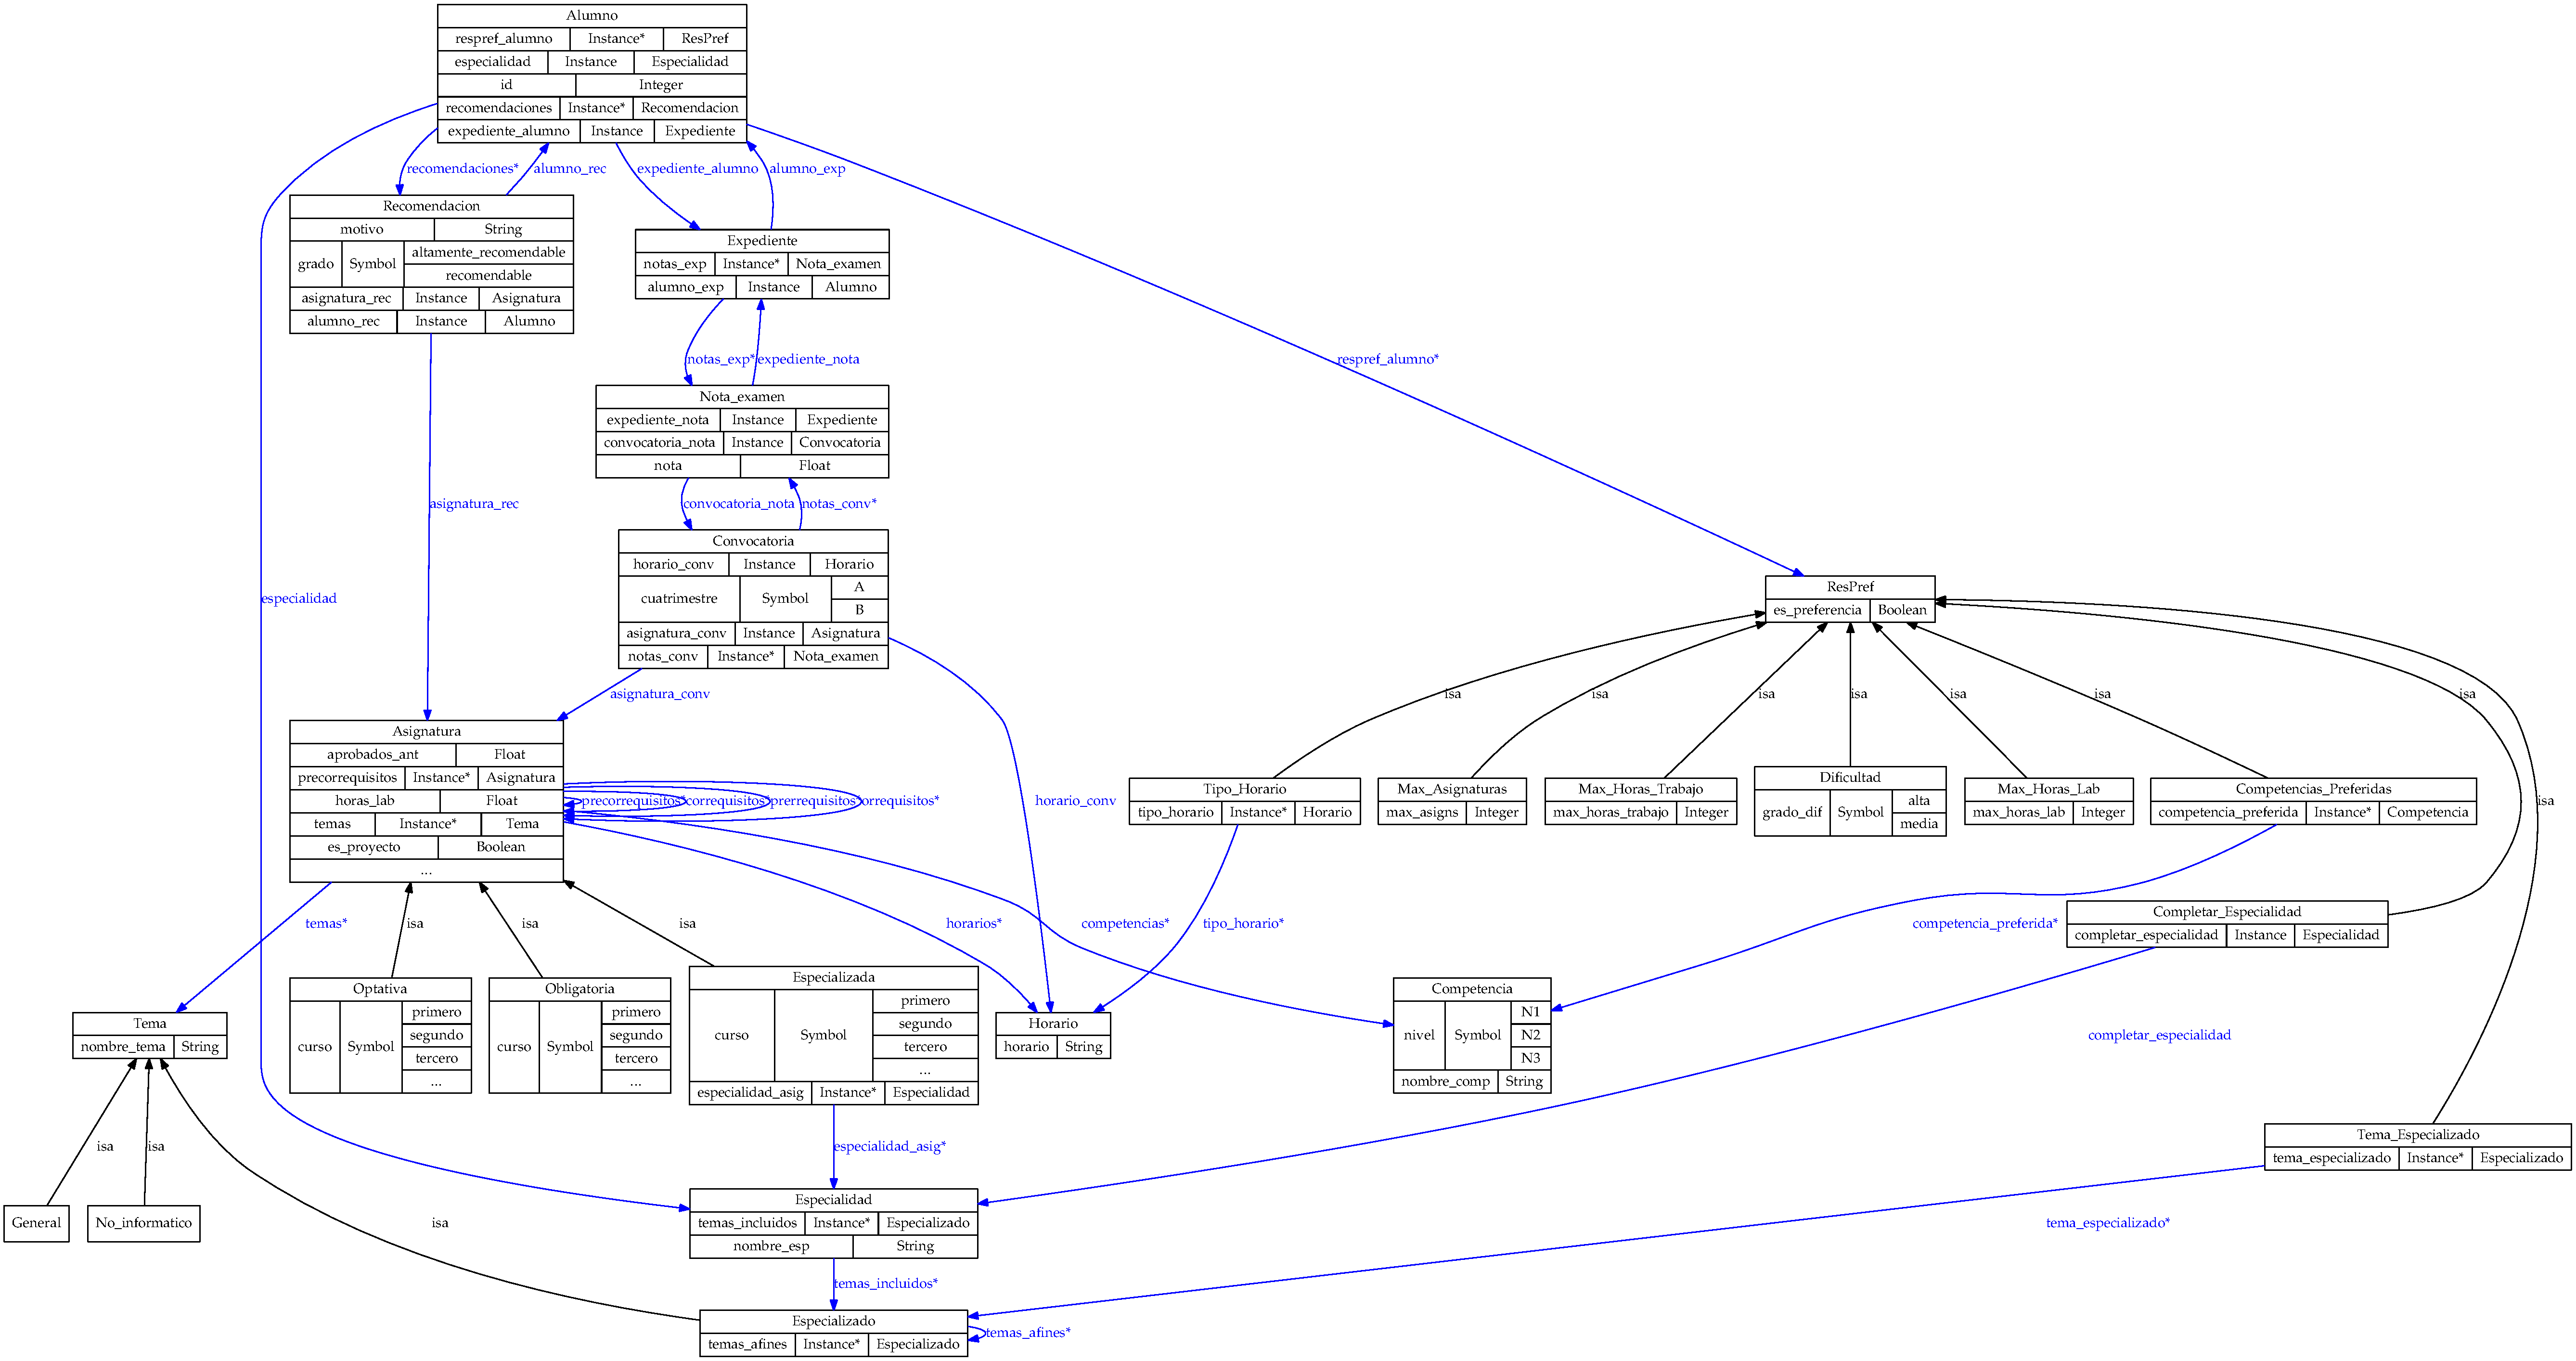
\includegraphics[width=23cm,height=14cm,keepaspectratio]{ontologia-completa}
        \caption{Representación gráfica de la ontología completa.}
        \label{fig:ontologia-completa}
    \end{figure}

\end{landscape}
}



\textbf{(grafo de jerarquía)}
